\documentclass[a4paper, 12pt]{article}
\usepackage[T1]{fontenc}
\usepackage{lmodern}
\usepackage{pdfpages}
\usepackage{color}
\usepackage{amsfonts}
\usepackage{epstopdf}
\usepackage{matlab}
%\documentclass{book}
\usepackage{blindtext}
\usepackage{hyperref}
\usepackage[brazil]{babel}
\usepackage{amssymb}
\usepackage[utf8]{inputenc}
\usepackage{amsmath}
\usepackage{indentfirst}
\usepackage{graphicx}
\usepackage{multicol,lipsum}
\usepackage[a4paper,
top=3cm, left=3cm, bottom=3cm, right=3cm]{geometry}
\usepackage{setspace}
\usepackage{multirow}
\usepackage{float}
\usepackage[dvipsnames]{xcolor}
\usepackage[table]{xcolor}
%\usepackage{pdflscape}
\usepackage[DIV=15]{typearea}
\usepackage[nottoc]{tocbibind}
\usepackage[sort,numbers]{natbib}
%\usepackage{cite}
\usepackage{matlab}

\usepackage[utf8]{inputenc}
\usepackage[T1]{fontenc}
\usepackage{lmodern}
\usepackage{graphicx}
\usepackage{color}
\usepackage{hyperref}
\usepackage{amsmath}
\usepackage{amsfonts}
\usepackage{epstopdf}
\usepackage[table]{xcolor}
\usepackage{matlab}


\documentclass[letterpaper]{article}
% bib pack %%%%%%%%%%%%%%%%%%%%%%%%%%%%%%%%%%%%%%%%%%%%%%%%%%%%%%%%%%%%%%%%%%%%%
\usepackage[utf8]{inputenc}
\usepackage{geometry}
    \geometry{left=3cm,right=2cm,top=2cm,bottom=2cm}
%
\usepackage[spanish]{babel}
%
\usepackage[fixlanguage]{babelbib}
    \bibliographystyle{babunsrt}
%
\usepackage{url}

\begin{document}
%\maketitle

\begin{titlepage}
	\begin{center}
		

\vspace{10pt}
%\begin{figure}[H][!ht]
%\centering
%
\includegraphics{puc-rio-logo.png}

%\end{figure}
\begin{figure}[!ht]
\centering

\includegraphics{images/puc-rio-logo.png}
\end{figure}
\huge{Fundamentos de Mecatrônica}
        \vspace{70pt}
        
		\textbf{ENG1731}
		\textbf{\large{\\ }}
		
		\vspace{30pt}
		\textbf{\small{\\Lista 04}}
		\vspace{75pt}
		
	\end{center}
	
	\begin{flushleft}
		\begin{tabbing}
		Aluno(a)\qquad\qquad\=\>Paloma Fernanda Loureiro Sette - 1621595\\
			
			Professor(a)\>João Carlos Virgolino Soares\\
	\end{tabbing}
		  
	\end{flushleft}
	\begin{center}
		%\vspace{\fill}
		\vspace{215pt}
		Rio de Janeiro, 01 de Junho de 2023
	\end{center}
\end{titlepage}
%%%%%%%%%%%%%%%%%%%%%%%%%%%%%%%%%%%%%%%%%%%%%%%%%%%%%%%%%%%
\newpage
\tableofcontents
\thispagestyle{empty}

\newpage
\pagenumbering{arabic}

\newpage

%\newcommand{\listequationsname}{Lista de Equações}
%\newlistof{myequations}{equ}{\listequationsname}
%\newcommand{\myequations}[1]{%
%\addcontentsline{equ}{myequations}{\protect\numberline{\theequation}#1}\par}

%\listofmyequations
\newpage


\newpage

\listoffigures
\thispagestyle{empty}

\newpage
%%%%%%%%%%%%%%%%%%%%%%%%%%%%%%%%%%%%%%%%%%%%%%%%%%%%%%%%%
%%%%%%%%%%%%%%%%%%%%%%%%%%%%%%%%%%%%%%%%%%%%%%%%%%%

\newpage

\thispagestyle{empty}

%%%%%%%%%%%%%%%%%%%%%%%%%%%%%%%%%%%%%%%%%%%%%%%%%%%%%%%%%%%%%%%%%%%%%%%
\newpage
\section{Introdução}
Este relatório refere-se ao quarto trabalho da disciplina de Fundamentos de Mecatrônica, ENG1731, de 2023.1. \\

Trataremos da simulação de um sistema mecânico do motor HC385MG-301, da Johnson, cujo datasheet é apresentado na página seguinte.

%%%%%%%%%%%%%%%%%%%%%%%%%%%%%%%%%%%%%%%%%%%%%%%%%%%%%%%%%%%%%%%%%%%%%%
\begin{center}
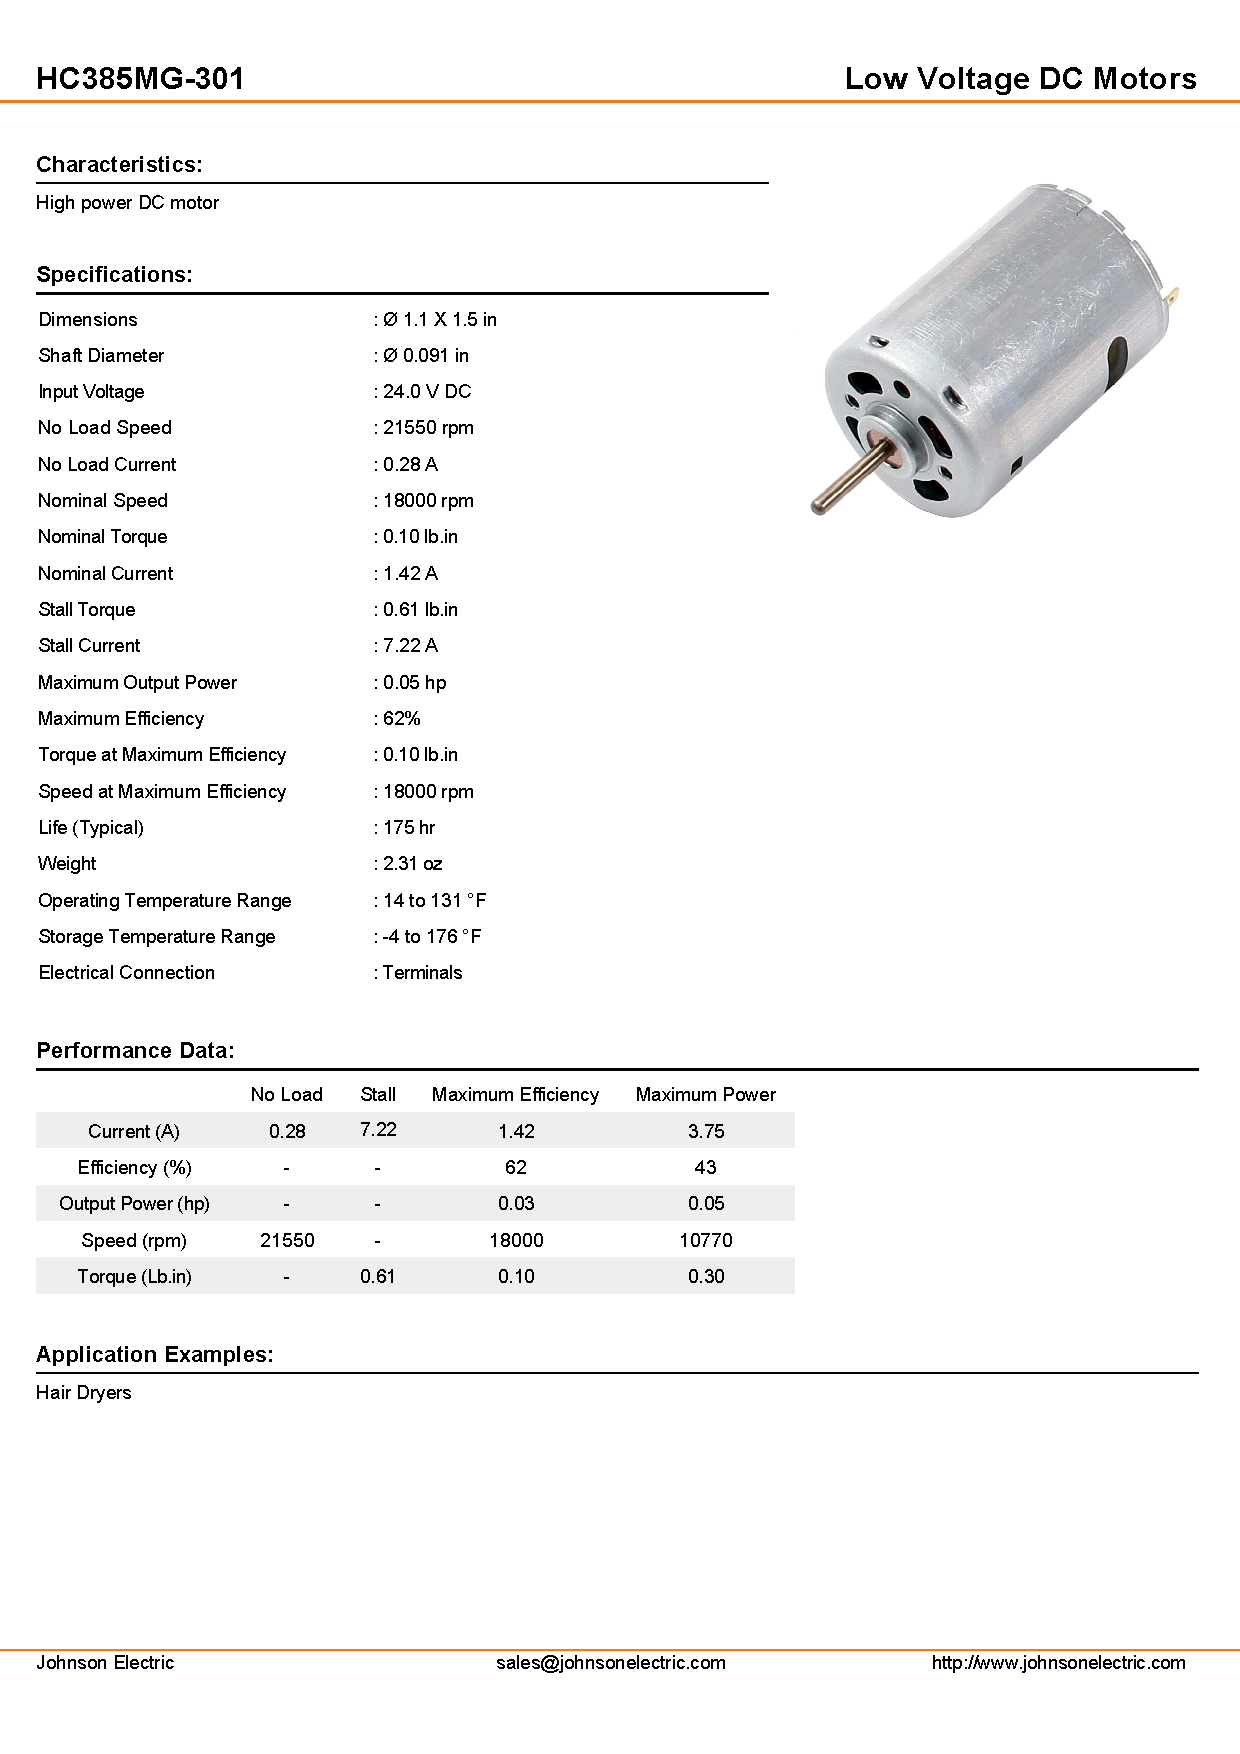
\includepdf[pagesize={6.5in,11in}]{motor_HC385MG-301_pg1.pdf}
\end{center}

O desenho técnico das dimensões são:

\begin{figure}[H]\label{desenho}
\centering
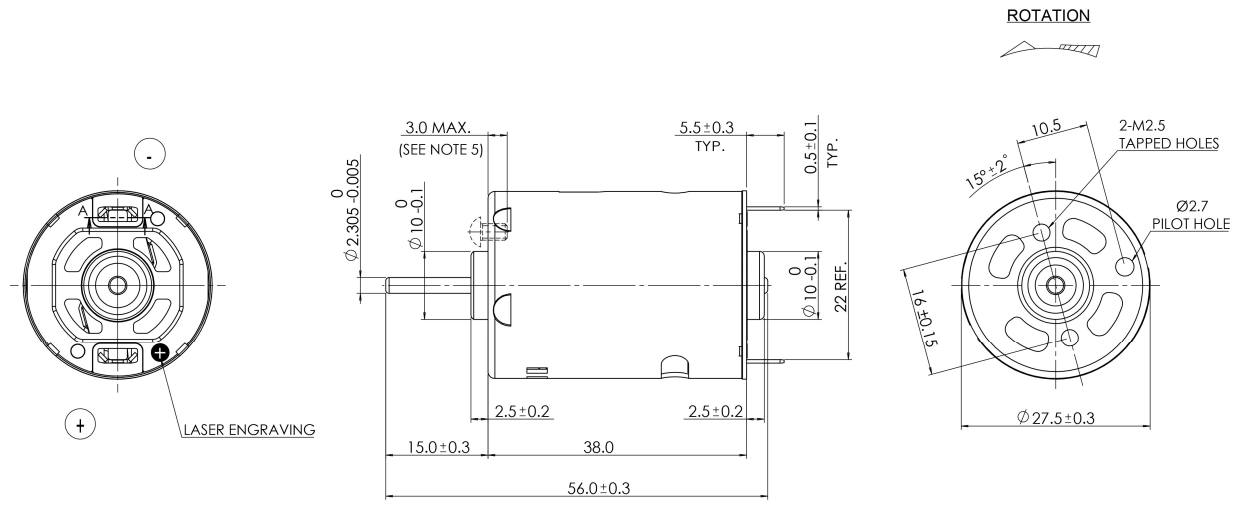
\includegraphics[scale = 0.5]{images/draw.png}
\label{filtro1}
\caption{Desenho técnico}
\end{figure}

E as curvas de performance são dadas a seguir:

\begin{figure}[H]\label{performance}
\centering
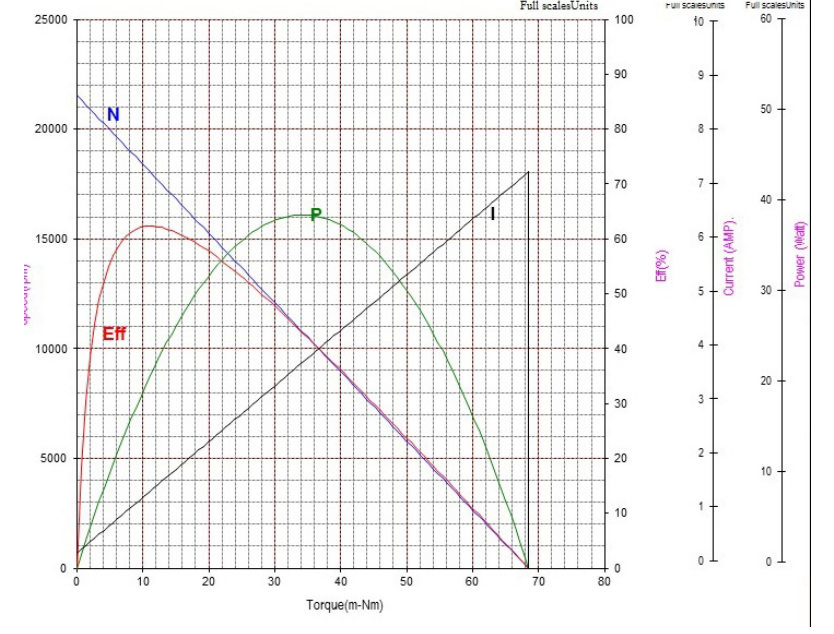
\includegraphics[scale = 0.7]{images/performance_curv.png}
\label{filtro1}
\caption{Curvas de Performance}
\end{figure}


%%%%%%%%%%%%%%%%%%%%%%%%%%%%%%%%%%%%%%%%%%%%%%%%%%%%%%%%%%%%%%%%%%%%%%


\newpage
\section{Questão 01}
\textbf{Selecionar no datasheet os parâmetros necessários para simular o comportamento do motor;} \\


Com base nos dados do datasheet fornecido para o motor HC385MG-301, os parâmetros necessários para simular o comportamento do motor são:



\begin{itemize}
    \item Tensão de entrada (Input Voltage): 24.0 V DC
    \item Velocidade sem carga (No Load Speed): 21550 rpm
    \item Corrente sem carga (No Load Current): 0.28 A
    \item Velocidade nominal (Nominal Speed): 18000 rpm
    \item Torque nominal (Nominal Torque): 0.10 lb.in
    \item Corrente nominal (Nominal Current): 1.42 A
    \item Torque de parada (Stall Torque): 0.61 lb.in
    \item Corrente de parada (Stall Current): 7.22 A
    \item Potência máxima de saída (Maximum Output Power): 0.05 hp
    \item Eficiência máxima (Maximum Efficiency): 62%
    \item Torque na máxima eficiência (Torque at Maximum Efficiency): 0.10 lb.in
    \item Velocidade na máxima eficiência (Speed at Maximum Efficiency): 18000 rpm
\end{itemize}

Esses parâmetros são necessários para caracterizar o comportamento do motor e podem ser utilizados em simulações ou análises de desempenho.\\

No entanto, por se tratar de um motor mais simples e barato, sabemos que alguns parâmetros que seriam relevantes costumam estar em falta no datasheet.\\

Pela imagem \ref{desenho}, podemos ver que $D = 1.1 in = 0.00254m$. Entao, da inércia do rotor ($J$), podemos tirar que

\begin{equation}
    J = \frac{1}{2}mR \>\ \longrightarrow \>\ J = \frac{1}{2} *65.49e^{-3}kg*(0.00254/2)^2
\end{equation}

E, também, sabemos que a potência de entrada , de saída e a eficiência são dadas, respectivamente, por:

\begin{equation}
    P_{in} = P_{el} = Vi
\end{equation}

\begin{equation}
    P_{out} = P_{mec} = T \omega
\end{equation}

\begin{equation}
    Ef = \frac{P_{out}}{P_{in}}
\end{equation}

%%%%%%%%%%%%%%%%%%%%%%%%%%%%%%%%%%%%%%%%%%%%%%%%%%%%%%%%%%%%%%%%%%%%%%%
\newpage
\section{Questão 02}


\textbf{Simule o comportamento dinâmico do motor escolhido no Simscape ou Simulink utilizando os parâmetros do datasheet.} \\

Foi utilizado o Simscape para a modelagem do motor referido. 

\begin{figure}[H]\label{performance}
\centering
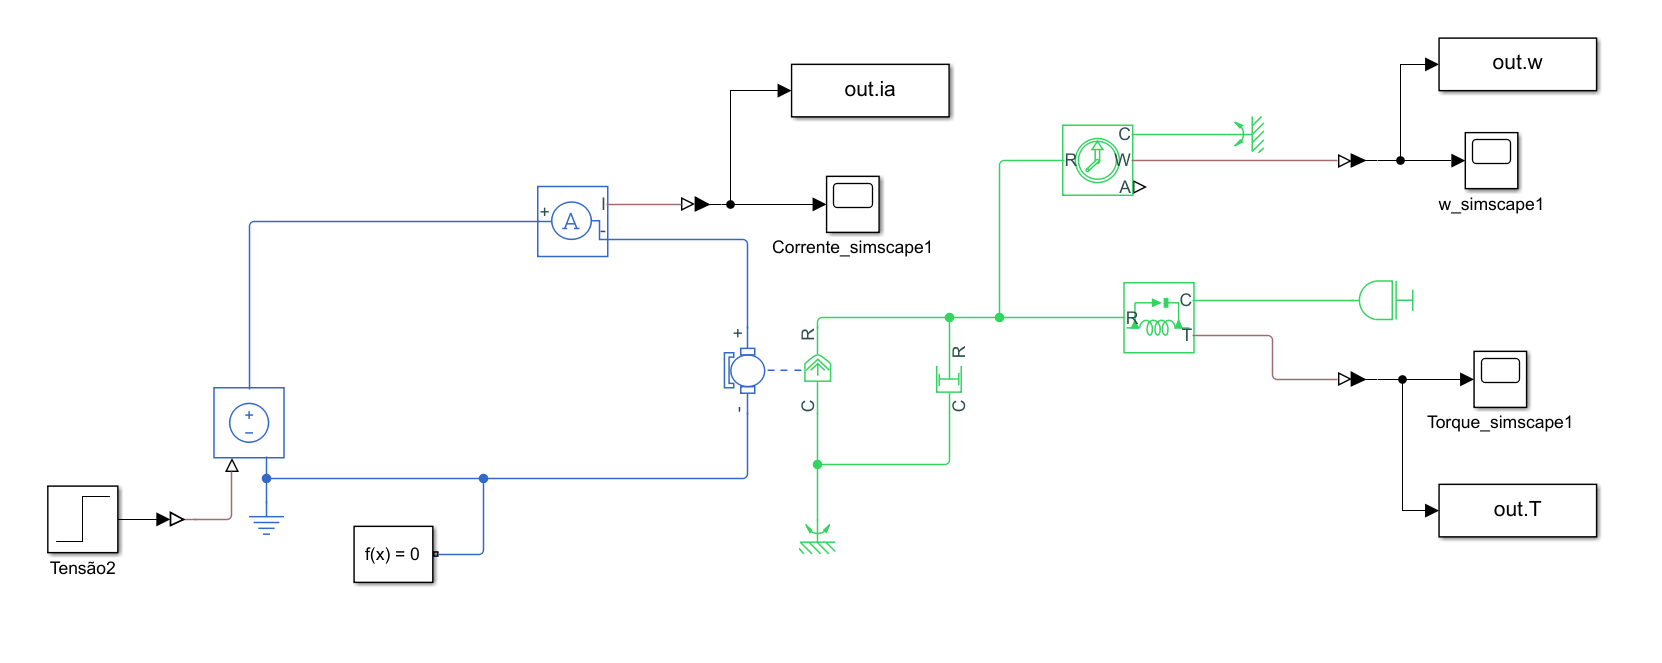
\includegraphics[scale = 0.35]{images/simscape2.png}
\label{filtro1}
\caption{Modelagem no Simscape}
\end{figure}

Abaixo, os gráficos gerados pelo modelo na simulação

\begin{figure}[H]\label{performance}
\centering
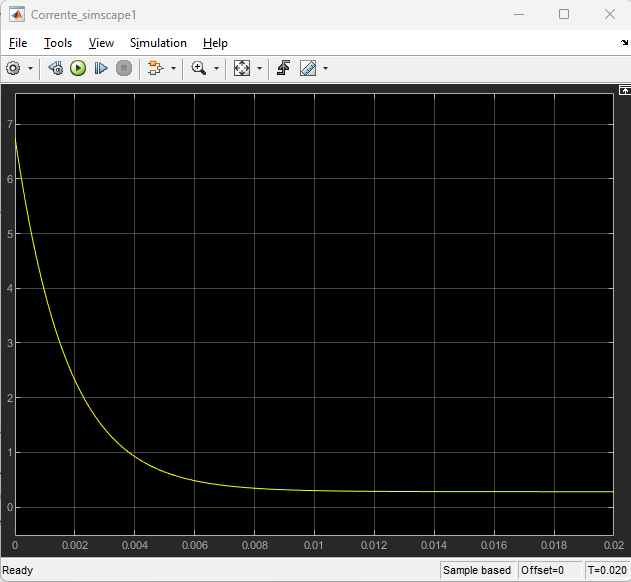
\includegraphics[scale = 0.60]{images/corrente_simscape.png}
\label{filtro1}
\caption{Gráfico da corrente em função do tempo gerado pelo Simscape}
\end{figure}

\begin{figure}[H]\label{performance}
\centering
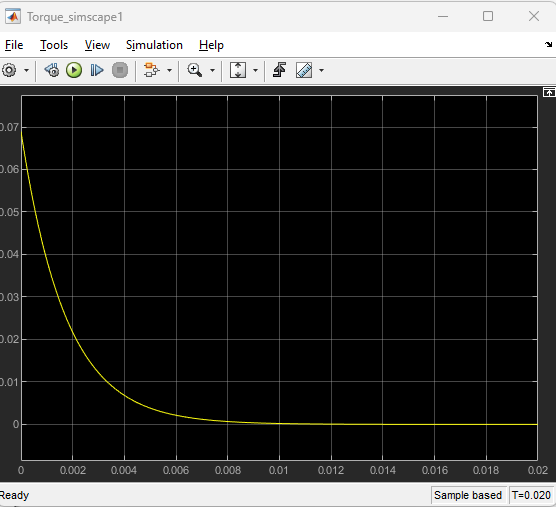
\includegraphics[scale = 0.65]{images/torque_simscape.png}
\label{filtro1}
\caption{Gráfico do torque em função do tempo gerado pelo Simscape}
\end{figure}

\begin{figure}[H]\label{performance}
\centering
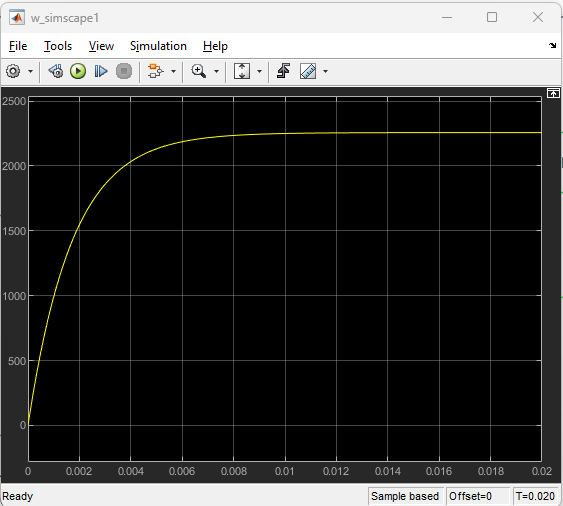
\includegraphics[scale = 0.65]{images/w_simscape.png}
\label{filtro1}
\caption{Gráfico da velocidade angular função do tempo gerado pelo Simscape}
\end{figure}
 
%%%%%%%%%%%%%%%%%%%%%%%%%%%%%%%%%%%%%%%%%%%%%%%%%%%%%%%%%%%%%%%%%%%%%%%%%
\newpage
\section{Questão 03}
\textbf{Gere as curvas de velocidade angular, torque de saída, corrente e potência mecânica em função do tempo. Não esqueça de colocar os nomes das variáveis nos eixos dos gráficos com a unidade correta. Compare os resultados com os dados do datasheet.}\\


Para a geração das curvas, foi utilizado o seguinte código no MATLAB:

\sloppy
\epstopdfsetup{outdir=./}
\graphicspath{ {./L01_Latex_images/} }

\begin{matlabcode}
% Parâmetros do motor
close all
clear
clc

speed_noload        = 21550*2*pi/60;    % rad/s
current_noload      = 0.28;             % A
stall_torque        = 0.06892;          % Nm

m   = 65.49e-3;
R   = 1.27e-3;
J = 0.5*m*R*R;

b   = 0;

Ea  = 24.0;

out = sim("simscape2_model_L04.slx");

t = out.tout;
T = out.T;
w = out.w;
ia = out.ia;

%%
Pmec = T.*w;
Pel = Ea*ia;
Ef = Pmec./Pel;

%%
figure

subplot(2, 3, 1)
plot(t, w*60/(2*pi))
grid on
title("Velocidade angular x Tempo")
xlabel("t [s]")
ylabel("w [rpm]")

subplot(2, 3, 2)
plot(t, ia)
grid on
title("Corrente x Tempo")
xlabel("t [s]")
ylabel("I [A]")

subplot(2, 3, 3)
plot(t, T)
grid on
title("Torque x Tempo")
xlabel("t [s]")
ylabel("T [Nm]")

subplot(2, 3, 4)
plot(t, Pmec)
grid on
title("Potencia mecanica x Tempo")
xlabel("t [s]")
ylabel("Pmec [W]")

subplot(2, 3, 5)
plot(t, Ef)
grid on
title("Eficiencia x Tempo")
xlabel("t [s]")
ylabel("eff [%]")

\end{matlabcode}

Ao final, foram geradas as seguintes curvas e podemos perceber que há coerência, embora haja uma pequena diferença entre os valores listados no datasheet e os respectivos valores simulados. 



\begin{figure}[H]\label{performance}
\centering
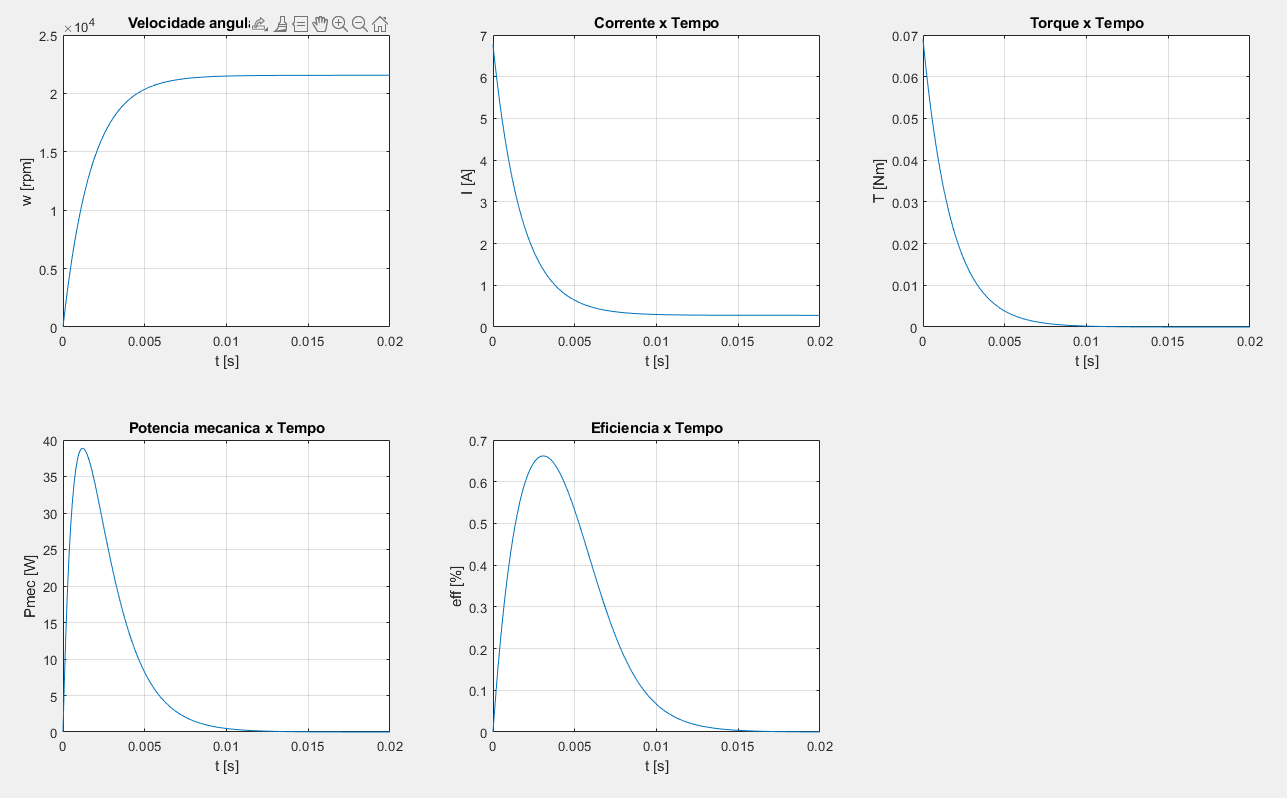
\includegraphics[scale = 0.45]{images/graficos_q03.png}
\label{filtro1}
\caption{Gráficos dos parâmetros em função do tempo}
\end{figure}

%%%%%%%%%%%%%%%%%%%%%%%%%%%%%%%%%%%%%%%%%%%%%%%%%%%%%%%%%%%%%%%%%%%%%%%%
\newpage
\section{Questão 04}
\textbf{ Gere as curvas de performance do motor em um script do MATLAB (corrente, velocidade angular, potência mecânica e eficiência em função do Torque). Não esqueça de colocar os nomes das variáveis nos eixos dos gráficos com a unidade correta.}\\

Foi utilizado o seguinte código para geração das curvas, onde foram modificados apenas alguns detalhes para que a geração das curvas pudessem estar em função do torque.

\sloppy
\epstopdfsetup{outdir=./}
\graphicspath{ {./L01_Latex_images/} }

\begin{matlabcode}
% Parâmetros do motor
close all
clear
clc

speed_noload        = 21550*2*pi/60;    % rad/s
current_noload      = 0.28;             % A
stall_torque        = 0.06892;          % Nm

m   = 65.49e-3;
R   = 1.27e-3;
J = 0.5*m*R*R;

b   = 0;

Ea  = 24.0;

out = sim("simscape2_model_L04.slx");

t = out.tout;
T = out.T;
w = out.w;
ia = out.ia;

%%
Pmec = T.*w;
Pel = Ea*ia;
Ef = Pmec./Pel;

%%
figure

subplot(2, 2, 1)
plot(T, w*60/(2*pi))
grid on
title("Velocidade angular x Torque")
xlabel("T [Nm]")
ylabel("w [rpm]")

subplot(2, 2, 2)
plot(T, ia)
grid on
title("Corrente x Torque")
xlabel("T [Nm]")
ylabel("I [A]")

subplot(2, 2, 3)
plot(T, Pmec)
grid on
title("Potencia mecanica x Torque")
xlabel("T [Nm]")
ylabel("Pmec [W]")

subplot(2, 2, 4)
plot(T, Ef)
grid on
title("Eficiencia x Torque")
xlabel("T [Nm]")
ylabel("eff [%]")
\end{matlabcode}

Ao final, foram geradas os seguintes gráficos que, comparando com os valores do datasheet, podemos dizer que estão fazendo sentido, embora haja uma pequena diferença entre o valor listado no datasheet e o respectivo parâmetro simulado. 

\begin{figure}[H]\label{performance}
\centering
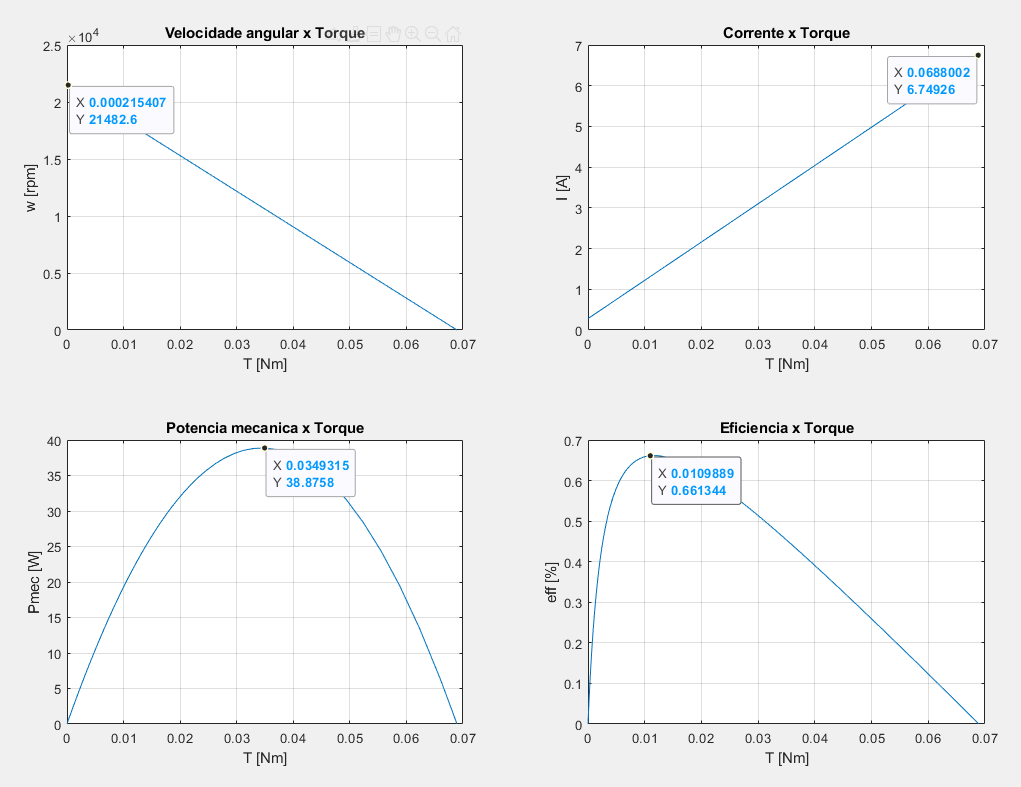
\includegraphics[scale = 0.50]{images/graficos_q04.png}
\label{filtro1}
\caption{Gráficos dos parâmetros em função do torque}
\end{figure}

%%%%%%%%%%%%%%%%%%%%%%%%%%%%%%%%%%%%%%%%%%%%%%%%%%%%%%%%%%%%%%%%%%%%%%%%%%%%
\newpage
\section{Questão 05}
\textbf{Compare as curvas de performance com os dados do datasheet, explicando o significado dos parâmetros.}\\

Vamos comparar as curvas de performance geradas pelo código com os dados do datasheet do motor HC385MG-301 e discutir o significado dos parâmetros.\\

\subsection{Curva de Velocidade Angular x Torque:}
A curva gerada mostra a relação entre a velocidade angular do motor (em rpm) e o torque aplicado (em Nm). Podemos observar que a velocidade angular diminui à medida que o torque aumenta, seguindo um comportamento esperado para um motor. A velocidade sem carga (no-load speed) mencionada no datasheet é de aproximadamente 21550 rpm, o que pode ser verificado na curva quando o torque é zero. Essa curva nos permite entender como a velocidade angular do motor varia de acordo com a carga aplicada.

\subsection{Curva de Corrente x Torque:}
Essa curva representa a relação entre a corrente elétrica fornecida ao motor (em A) e o torque aplicado (em Nm). Podemos observar que a corrente aumenta à medida que o torque aumenta, o que é esperado, uma vez que a corrente é proporcional ao torque para um motor DC. A corrente sem carga (no-load current) mencionada no datasheet é de 0.28 A, o que pode ser verificado na curva quando o torque é zero. Essa curva nos permite entender como a corrente elétrica varia em função do torque aplicado.

\subsection{Curva de Potência Mecânica x Torque:}
Essa curva representa a potência mecânica desenvolvida pelo motor (em W) em função do torque aplicado (em Nm). Podemos observar que a potência mecânica aumenta à medida que o torque aumenta, até atingir um valor máximo e, em seguida, diminui. O valor máximo da potência mecânica ocorre quando o torque corresponde ao torque de potência máxima, que é aproximadamente 0.0345 Nm, conforme calculado anteriormente. Esse valor pode ser comparado com o valor máximo de potência mencionado no datasheet, que é de 0.05 hp (ou aproximadamente 37.3 W).

\subsection{Curva de Eficiência x Torque:}
Essa curva representa a eficiência do motor (em \%) em função do torque aplicado (em Nm). Podemos observar que a eficiência é máxima em torno de 62\%, conforme mencionado no datasheet. A eficiência é calculada dividindo-se a potência mecânica pela potência elétrica de entrada (Pel = Ea * ia). Portanto, a curva de eficiência nos permite entender como a eficiência do motor varia em diferentes cargas.\\

Em resumo, as curvas de performance geradas pelo código estão de acordo com os dados do datasheet em termos de tendências gerais. Elas nos ajudam a compreender como o motor HC385MG-301 se comporta em relação à velocidade angular, corrente, potência mecânica e eficiência, conforme diferentes torques são aplicados.


%%%%%%%%%%%%%%%%%%%%%%%%%%%%%%%%%%%%%%%%%%%%%%%%%%%%%%%%%%%%%%%%%%%%%%%%%
\newpage
\section{Questão 06}
\textbf{Calcule o torque correspondente à potência máxima usando os parâmetros de performance do motor.}\\

Podemos analisar matematicamente. Sabemos que

\begin{equation}
    T = K_T i_a = \frac{K_T}{R_a}e_a - \frac{K_TK_e}{R_a}\frac{d\theta}{dt}
\end{equation}

Onde $\frac{K_T}{R_a} = K_V$ e $\frac{K_TK_e}{R_a} = K_\omega$ \\ 

Logo, 

\begin{equation}\label{eq}
    T = K_VV - K_\omega \omega
\end{equation}

O $K_V$ pode ser interpretado como a capacidade de geração de torque a partir da tensão de alimentação. Já o $K_\omega$ pode ser interpretado como a dissipação interna total, combinado à energia eletromecânica, que é o quanto irá diminuir do torque final. A unidade de $K_V$ é [Nm/V] e a unidade de $K_\omega$ é [Nm/rad/s]. 

Então, a partir disso, podemos analisar alguns fatores em relação à potência mecânica. 

Portanto, para $T = 0$, teremos

\begin{equation}
    K_VV = K_\omega \omega_0 \>\ \longrightarrow \>\ \omega_0 = \frac{K_V}{K_\omega} V
\end{equation}

multiplicando toda a equação \ref{eq} por $\frac{1}{k_\omega}$, teremos que

\begin{equation}
    \omega = \omega_0 - \frac{1}{K_\omega} T^2
\end{equation}

Então, temos uma função que descreve o comportamento da velocidade do sistema em função da velocidade máxima menos uma constante vezes o torque. Logo, podemos usar isso para calcular a potência, pois a potência mecânica é dada por $P_{mec} = T\omega$, logo

\begin{equation}
    P_{mec} = \omega_0T - \frac{1}{K_\omega}T^2
\end{equation}


Portanto, para sabermos o torque cuja potência é máxima, fazemos

\begin{equation}
    \frac{dP_{mec}}{dT} = \omega_0 - \frac{2}{K_\omega}T = 0
\end{equation}

Logo, 

\begin{equation}
      T = \frac{\omega_0 K_\omega}{2}
\end{equation}

E o valor da potência máxima, consequentemente, seria:

\begin{equation}\label{pmax}
      P_{max} = \frac{\omega_0^2 K_\omega}{4}
\end{equation}

No entanto, podemos fazer algumas considerações. Sabemos que $T = T = K_VV - K_\omega \omega$ e que se $\omega =0$, então temos $T = T_{stall}$. Então, $T_{stall} = K_VV$. Logo, 

\begin{equation}
    \omega_0 = \frac{T_{stall}}{K_\omega} \>\ \longrightarrow \>\ K_\omega = \frac{T_{stall}}{\omega_0}
\end{equation}



Sabemos, neste caso, que a potência máxima, bem como o torque relativo à mesma, irá depender da velocidade angular sem carga  (No Load Current) e do torque de stall (Stall Torque). Logo, analisando os valores do datasheet, nosso torque relativo à potência máxima será

\begin{equation}
      T = \frac{\omega_0 \frac{T_{stall}}{\omega_0} }{2} = \frac{T_{stall}}{2} = 0.0345Nm
\end{equation}\\ \\









%%%%%%%%%%%%%%%%%%%%%%%%%%%%%%%%%%%%%%%%%%%%%%%%%%%%%%%%%%%%%%%%%%%%%%%%%
\newpage
\section{Questão 07}
\textbf{ Encontre o valor máximo do vetor de potência mecânica (sugestão: usar o comando max do MATLAB). Compare o valor com o encontrado no item 6.}\\

Pelo MATLAB, reescrevemos o código da seguinte maneira:


\sloppy
\epstopdfsetup{outdir=./}
\graphicspath{ {./L01_Latex_images/} }

\begin{matlabcode}

% Parâmetros do motor
Ea              = 24.0;          % V
speed_noload    = 21550*2*pi/60; % (rad/s)
current_noload  = 0.28;          % A
stall_torque    = 0.0689;        % Nm
stall_current   = 7.22;          % A

% Cálculo do torque correspondente à potência máxima
omega0      = speed_noload;
K_omega     = stall_torque / omega0;
T_pmax      = stall_torque / 2;

% Definição do vetor de torque
torque      = 0:0.0001:stall_torque;

% Cálculo da potência mecânica
P_mec       = omega0 * torque - (1 / K_omega) * torque.^2;

% Encontrando o valor máximo da potência mecânica
[P_max, indexMax]   = max(P_mec);
T_max               = torque(indexMax);

%% Plot das curvas
figure;
plot(torque, P_mec);
hold on;
plot([T_pmax T_pmax], [0 P_max], 'r--');
hold off;
xlabel('Torque (Nm)');
ylabel('Potência Mecânica (W)');

% Exibir o valor máximo da potência mecânica e torque correspondente
disp(['Valor máximo da potência mecânica: ', num2str(P_max), ' W']);
disp(['Torque correspondente à potência máxima: ', num2str(T_max), ' Nm']);

\end{matlabcode}

E geramos a curva abaixo.


\begin{figure}[H]\label{desenho}
\centering
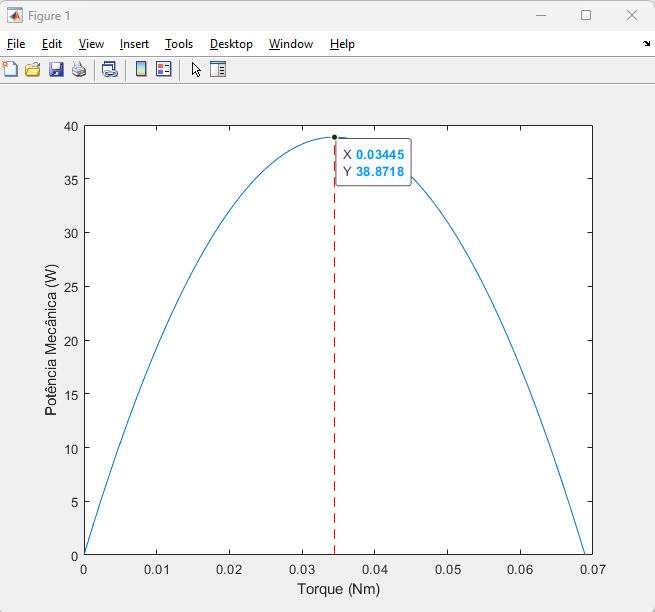
\includegraphics[scale = 0.7]{images/q07.png}
\label{filtro1}
\caption{Questao 07: curva gerada pelo MATLAB}
\end{figure}


Analisando o resultado da plotagem, podemos notar que há coerência do valor do torque com o resultado gerado na questão anterior, onde pedia, matematicamente, o valor do torque relativo à potência máxima. 

Podemos notar, além disso, que o valor máximo da potência está coerente com o que nos forneceu o datasheet, pois há proximidade nos valores (podemos comparar, observando a imagem \ref{performance}).








\newpage
% REFERENCIAS %%%%%%%%%%%%%%%%%%%%%%%%%%%%%%%%%%%%%%%%%%%%%%%%%%%%%%%%%%%%%%
    \nocite{*}
    \bibliography{src/bibliography}
    
\end{document}
\section{Referências Bibliográficas}



\end{document}